\documentclass[mathserif]{beamer}

\setbeamertemplate{frametitle}[default][center]%Centers the frame title.
\setbeamertemplate{navigation symbols}{}%Removes navigation symbols.
\setbeamertemplate{footline}{\raisebox{5pt}{\makebox[\paperwidth]{\hfill\makebox[10pt]{\scriptsize\insertframenumber}}}}

\usepackage{amsmath,amssymb,amsthm,amsfonts}
\usepackage{nicefrac}
\usepackage{graphicx,array,dsfont}
\usepackage{wrapfig}
\usepackage{harvard}
\usepackage{multirow}
\citationmode{abbr}

\newcommand{\Hrule}{\rule{\linewidth}{0.2pt}}
\newcommand{\argmax}{\mathop{\mathrm{argmax}}}
\newcommand{\argmin}{\mathop{\mathrm{argmin}}}
\newcommand{\minimize}{\mathop{\mathrm{minimize}}}
\def\half{\frac{1}{2}}
\def\th{\mathrm{th}}
\def\sign{\mathrm{sign}}
\def\supp{\mathrm{supp}}
\def\E{\mathrm{E}}
\def\P{\mathrm{P}}
\def\Var{\mathrm{Var}}
\def\Cov{\mathrm{Cov}}
\def\Cor{\mathrm{Cor}}
\def\var{\mathrm{var}}
\def\cov{\mathrm{cov}}
\def\cor{\mathrm{cor}}
\def\rcor{\mathrm{rcor}}
\def\mcor{\mathrm{mcor}}
\def\mCor{\mathrm{mCor}}
\def\dCov{\mathrm{dCov}}
\def\dcov{\mathrm{dcov}}
\def\dVar{\mathrm{dVar}}
\def\dvar{\mathrm{dvar}}
\def\dCor{\mathrm{dCor}}
\def\dcor{\mathrm{dcor}}
\def\trace{\mathrm{trace}}
\def\col{\mathrm{col}}
\def\R{\mathds{R}} 
\def\cA{\mathcal{A}}
\def\cB{\mathcal{B}}
\def\cE{\mathcal{E}}
\def\cF{\mathcal{F}}
\def\cG{\mathcal{G}}
\def\cN{\mathcal{N}}
\def\hbeta{\hat{\beta}}
\def\hy{\hat{y}}
\def\red{\color[rgb]{0.8,0,0}}
\def\white{\color[rgb]{1,1,1}}
\def\blue{\color[rgb]{0,0,0.8}}
\def\green{\color[rgb]{0,0.4,0}}

\begin{document}

\title{Classification 1: Linear regression of indicators,
linear discriminant analysis}
\author{Ryan Tibshirani \\ Data Mining: 36-462/36-662}
\date{April 2 2013}

\begin{frame}
\maketitle
{\it Optional reading: ISL 4.1, 4.2, 4.4, ESL 4.1--4.3}
\end{frame}

\begin{frame}
\frametitle{Classification}
{\red Classification} is a predictive task in which the response takes
values across discrete categories (i.e., not continuous), and in the 
most fundamental case, two categories

\bigskip
Examples:
\begin{itemize}
\item Predicting whether a patient will develop breast cancer or remain
healthy, given genetic information
\item Predicting whether or not a user will like a new product, based on
user covariates and a history of his/her previous ratings
\item Predicting the region of Italy in which a brand of olive oil was 
made, based on its chemical composition
\item Predicting the next elected president, based on various social,
political, and historical measurements
\end{itemize}
\end{frame}

\begin{frame}
\frametitle{}
Similar to our usual setup, we observe pairs $(x_i,y_i)$, $i=1,\ldots n$, 
where $y_i$ gives the class of the $i$th observation, and $x_i \in \R^p$ are
the measurements of $p$ predictor variables

\bigskip
Though the class labels may actually be $y_i \in \{\mathrm{healthy}, 
\mathrm{sick}\}$ or $y_i \in \{\mathrm{Sardinia}, \mathrm{Sicily}, ... \}$, 
but we can always encode them as 
$$y_i \in \{1,2,\ldots K\}$$
where $K$ is the total number of classes

\bigskip
Note that there is a {\red big difference} between classification and
clustering; in the latter, there is not a pre-defined notion of class 
membership (and sometimes, not even $K$), and we are not given labeled 
examples $(x_i,y_i)$, $i=1,\ldots n$, but only $x_i$, $i=1,\ldots n$
\end{frame}

\begin{frame}
\frametitle{}
Constructed from training data $(x_i,y_i)$, $i=1,\ldots n$, we denote our 
classification rule by $\hat{f}(x)$; given any $x \in \R^p$, this returns a 
class label $\hat{f}(x) \in \{1,\ldots K\}$

\bigskip
As before, we will see that there are two different ways of assessing the quality 
of $\hat{f}$: its {\red predictive ability} and {\red interpretative ability}

\bigskip
\begin{tabular}{cc}
\parbox{0.5\textwidth}{
E.g., train on $(x_i,y_i)$, $i=1,\ldots n$, the data of elected presidents
and related feature measurements $x_i \in \R^p$ for the past $n$ elections,
and predict, given the current feature measurements $x_0 \in \R^p$, the winner 
of the current election}&
\hspace{3pt}
\parbox{0.35\textwidth}{
\includegraphics[width=0.35\textwidth]{candidates.jpg}
}
\end{tabular}

\bigskip
In what situations would we care more about prediction error? And in what 
situations more about interpretation?
\end{frame}

\begin{frame}
\frametitle{Binary classification and linear regression}
Let's start off by supposing that $K=2$, so that the response is 
$y_i \in \{1,2\}$, for $i=1,\ldots n$

\bigskip
You already know a tool that you could potentially use in this case for classification:
{\red linear regression}. Simply treat the response
as if it were continuous, and find the linear regression coefficients 
of the response vector $y \in \R^n$ onto the predictors, i.e., 
$$\hbeta_0, \hbeta = \argmin_{\beta_0\in\R, \,\beta \in \R^p} \, 
\sum_{i=1}^n (y_i - \beta_0 - x_i^T \beta)^2 $$

Then, given a new input $x_0 \in \R^p$, we predict the class to be
$$\hat{f}^\mathrm{LS}(x_0) = \begin{cases}
1 & \mathrm{if}\; \hbeta_0 + x_0^T \hbeta \leq 1.5 \\
2 & \mathrm{if}\; \hbeta_0 + x_0^T \hbeta  > 1.5
\end{cases}$$
\end{frame}

\begin{frame}
\frametitle{}
(Note: since we included an intercept term in the regression, it doesn't
matter whether we code the class labels as $\{1,2\}$ or $\{0,1\}$, etc.)

\bigskip
In many instances, this actually works reasonably well. Examples:

\bigskip
\includegraphics[width=0.33\textwidth]{lin1.pdf}
\includegraphics[width=0.33\textwidth]{lin2.pdf}
\includegraphics[width=0.33\textwidth]{lin3.pdf}
%For the last example, there is a split that achieves only 12 mistakes

\bigskip
Overall, using linear regression in this way for binary classification is not 
a crazy idea. But how about if there are more than 2 classes?
\end{frame}

\begin{frame}
\frametitle{Linear regression of indicators}
This idea extends to the case of more than two classes. Given $K$ classes,
define the {\red indicator matrix} $Y \in \R^{n\times K}$ to be the matrix
whose columns indicate class membership; that is, its $j$th column satisfies
$Y_{ij} = 1$ if $y_i=j$ (observation $i$ is in class $j$) and $Y_{ij}=0$ 
otherwise

\bigskip
E.g., with $n=6$ observations and $K=3$ classes, the matrix 
$$Y = 
\left(\begin{array}{ccc}
1 & 0 & 0 \\
1 & 0 & 0 \\
0 & 1 & 0 \\
0 & 1 & 0 \\
0 & 0 & 1 \\
0 & 0 & 1 \\
\end{array}\right) \in \R^{6 \times 3}$$
corresponds to having the first two observations in class 1, the next two
in class 2, and the final 2 in class 3
\end{frame}

\begin{frame}
\frametitle{}
To construct a prediction rule, we regress 
each column $Y_j \in \R^n$ (indicating the $j$th class versus all else)
onto the predictors:
$$\hbeta_{j,0}, \hbeta_j = \argmin_{\beta_{j,0}\in\R,\,\beta_j \in \R^p} 
\, \sum_{i=1}^n (Y_{ij} - \beta_{0,j} - \beta_j^T x_i)^2$$

Now, given a new input $x_0 \in \R^p$, we compute
$$\hbeta_{0,j} + x_0^T \hbeta_j, \;\;\; j=1,\ldots K$$
take predict the class $j$ that corresponds to the highest score. I.e., we let
each of the $K$ linear models {\red make its own prediction}, and then we take 
the strongest. Formally, $$\hat{f}^\mathrm{LS}(x_0) = 
\argmax_{j=1,\ldots K} \; \hbeta_{0,j} + x_0^T \hbeta_j $$
\end{frame}

\begin{frame}
\frametitle{}
The {\red decision boundary} between any two classes $j,k$ are the values of
$x \in \R^p$ for which 
$$\hbeta_{0,j} + x^T \hbeta_j  = \hbeta_{0,k} + x^T \hbeta_k$$
i.e., $\hbeta_{0,j}-\hbeta_{0,k} + (\hbeta_j-\hbeta_k)^T x = 0$

\bigskip
\bigskip
\begin{tabular}{cc}
\parbox{0.475\textwidth}{
\includegraphics[width=0.475\textwidth]{blank.png}}
%\includegraphics[width=0.475\textwidth]{db.png}}
\hspace{-15pt}
\parbox{0.5\textwidth}{
This defines a $(p-1)$-dimensional affine subspace in $\R^p$. 
% it's actually affine if we include intercept
To one side, we would always predict class $j$
over $k$; to the other, we would always predict class $k$ over $j$}
\end{tabular}

\bigskip
\bigskip
\bigskip
For $K$ classes total, there are ${K \choose 2}=\frac{K(K-1)}{2}$ decision boundaries
\end{frame}

\begin{frame}
\frametitle{Ideal result}
\smallskip
What we'd like to see when we use linear regression for a
3-way classification (from ESL page 105):
\vspace{-2pt}
\begin{center}
\includegraphics[width=2.25in]{ideal.png}
\end{center}
\vspace{-5pt}
The plotted lines are the decision boundaries between classes 1 and 2, and 2 and 3
(the decision boundary between classes 1 and 3 never matters)
\end{frame}

\begin{frame}
\frametitle{Actual result}
\smallskip
What actually happens when we use linear regression for this 3-way classification
(from ESL page 105):
\begin{center}
\includegraphics[width=2.20in]{actual.png}
\end{center}
\vspace{-5pt}
The decision boundaries between 1 and 2 and between 2 and 3 are the same, so we 
would never predict class 2. This problem is called {\red masking} (and it is not
uncommon for moderate $K$ and small $p$)
\end{frame}

\begin{frame}
\frametitle{Why did this happen?}
Projecting onto the line joining the three class centroids gives some insight into 
why this happened (from ESL page 106):
\begin{center}
\includegraphics[width=2.6in]{why.png}
\end{center}
\end{frame}

\begin{frame}
\frametitle{Statistical decision theory}
\smallskip
\smallskip
%%% CHANGE C HERE AND HEREAFTER TO Y
Let $C$ be a random variable giving the class label of an 
observation in our data set. A natural rule would be to classify 
according to 
$$f(x) = \argmax_{j=1,\ldots K} \; \P(C=j|X=x)$$
This predicts the most likely class, given the feature measurements $X=x \in \R^p$.
This is called the {\red Bayes classifier}, and it is the best that we can do (think 
of overlapping classes)

\bigskip
Note that we can use Bayes' rule to write
$$\P(C=j|X=x) = \frac{\P(X=x|C=j) \cdot \P(C=j)}
{\P(X=x)}$$
Let $\pi_j = \P(C=j)$ be the {\red prior probability} of class $j$.
Since the Bayes classifier compares the above quantity across $j=1,\ldots K$ 
for $X=x$, the denominator is always the same, hence
$$f(x) = \argmax_{j=1,\ldots K}\; \P(X=x|C=j) \cdot \pi_j$$
\end{frame}

\begin{frame}
\frametitle{Linear discriminant analysis}
Using the Bayes classifier is not realistic as it requires knowing the 
class conditional densities $\P(X=x|C=j)$ and prior probabilities $\pi_j$. 
But if estimate these quantities, then we can follow the idea

\bigskip
{\red Linear discriminant analysis} (LDA) does this by assuming that 
the data within each class are normally distributed: 
$$h_j(x) = \P(X=x|C=j) = N(\mu_j, \Sigma) \;\mathrm{density} $$
We allow each class to have {\red its own mean} $\mu_j \in \R^p$, but 
we assume a {\red common covariance matrix} $\Sigma \in \R^{p \times p}$.
Hence
$$h_j(x) = \frac{1}{(2\pi)^{p/2} \mathrm{det}(\Sigma)^{1/2}}
\exp\Big\{-\frac{1}{2}(x-\mu_j)^T \Sigma^{-1} (x-\mu_j)\Big\}$$
So we want to find $j$ so that $\P(C=j|X=x)\cdot\pi_j =
h_j(x)\cdot\pi_j$ is the largest

%(Note that here it is key to assume that $X$ is random, whereas in linear
%regression we consider $X$ fixed.)
\end{frame}

\begin{frame}
\frametitle{}
\smallskip
Since $\log(\cdot)$ is a monotone function, we can consider maximizing
$\log(h_j(x) \pi_j)$ over $j=1,\ldots K$. We can define the rule:
\begin{align*}
f^\mathrm{LDA}(x) \;\;\;&=\;\;\;
\argmax_{j=1,\ldots K} \; \hspace{150pt} \\
\;\;\;&=\;\;\; 
\argmax_{j=1,\ldots K} \; \hspace{150pt} \\
\;\;\;&=\;\;\; 
\argmax_{j=1,\ldots K} \; \hspace{150pt} \\
\;\;\;&=\;\;\; 
\argmax_{j=1,\ldots K} \; \delta_j(x) 
\end{align*} 

\bigskip
We call $\delta_j(x)$, $j=1,\ldots K$ the {\red discriminant functions}. Note
$$\delta_j(x) = x^T \Sigma^{-1} \mu_j - \frac{1}{2}\mu_j^T \Sigma^{-1} 
\mu_j + \log\pi_j $$
is just an affine function of $x$
\end{frame}

\begin{frame}
\frametitle{}
\bigskip
In practice, given an input $x\in\R^p$, can we just use the rule 
$f^\mathrm{LDA}$ on the previous slide?
Not quite! What's missing: we don't know $\pi_j$, $\mu_j$, and $\Sigma$. Therefore 
we {\red estimate them} based on the training data $x_i \in \R^p$ and 
$y_i \in \{1,\ldots K\}$, $i=1,\ldots n$, by:
\smallskip
\begin{itemize}
\item $\hat{\pi}_j = n_j/n$, the proportion of observations in class $j$
\item $\hat{\mu}_j = \frac{1}{n_j} \sum_{y_i=j} x_i$, the centroid of class $j$
\item $\hat{\Sigma} = \frac{1}{n-K} \sum_{j=1}^K \sum_{y_i=j} 
(x_i - \hat{\mu}_j)(x_i - \hat{\mu}_j)^T$, the pooled sample covariance matrix
\end{itemize}
(Here $n_j$ is the number of points in class $j$)

\bigskip
This gives the estimated discriminant functions:
$$\hat{\delta}_j(x) = x^T \hat{\Sigma}^{-1} \hat{\mu}_j - 
\frac{1}{2}\hat{\mu}_j^T \hat{\Sigma}^{-1}\hat{\mu}_j + \log\hat{\pi}_j$$
and finally the linear discriminant analysis rule,
$$\hat{f}^\mathrm{LDA}(x) = \argmax_{j=1,\ldots K} \; \hat{\delta}_j(x)$$
\end{frame}

\begin{frame}
\frametitle{LDA decision boundaries}
The estimated discriminant functions
\begin{align*}
\hat{\delta}_j(x) &= x^T \hat{\Sigma}^{-1} \hat{\mu}_j - 
\frac{1}{2}\hat{\mu}_j^T \hat{\Sigma}^{-1}\hat{\mu}_j + \log\hat{\pi}_j \\
&= a_j + b_j^T x
\end{align*}
are just affine functions of $x$. 
The {\red decision boundary} between classes $j,k$ is the set of all 
$x \in \R^p$ such that $\hat{\delta}_j(x)=\hat{\delta}_k(x)$, i.e.,
$$a_j + b_j^T x = a_k + b_k^T x$$

\bigskip
\begin{tabular}{cc}
\parbox{0.45\textwidth}{
This defines an affine subspace in $x$:
$$ a_j-a_k + (b_j-b_k)^T x = 0 $$} &
\parbox{0.4\textwidth}{
\includegraphics[width=0.5\textwidth]{blank.png}}
\end{tabular}
\end{frame}

\begin{frame}
\frametitle{Example: LDA decision boundaries}
Example of decision boundaries from LDA (from ESL page 109):
\begin{center}
$f^\mathrm{LDA}(x)$ \hspace{1.5in} $\hat{f}^\mathrm{LDA}(x)$ \\
\smallskip
\includegraphics[width=4in]{ldaex.png}
\end{center} 
Are the decision boundaries the same as the perpendicular 
bisectors (Voronoi boundaries) between the class centroids?
(Why not?)
\end{frame}

\begin{frame}
\frametitle{LDA computations, usages, extensions}
The decision boundaries for LDA are useful for graphical 
purposes, but to classify a new point $x_0 \in \R^p$ we don't
use them---we simply compute $\hat{\delta}_j(x_0)$ for each 
$j=1,\ldots K$

\bigskip
LDA performs quite well on a wide variety of data sets, even when
pitted against fancy alternative classification schemes. Though
it assumes normality, its simplicity often works in its favor.
(Why? Think of the {\red bias-variance tradeoff})

\bigskip
Still, there are some useful extensions of LDA. E.g.,
\begin{itemize}
\item {\red Quadratic discriminant analysis}: using the same normal model,
we now allow each class $j$ to have its own covariance matrix $\Sigma_j$.
This leads to quadratic decision boundaries
\item {\red Reduced-rank linear discriminant analysis}: we essentially 
project the data to a lower dimensional subspace before performing LDA.
We will study this next time
\end{itemize}
\end{frame}

\begin{frame}
\frametitle{Example: olive oil data}
\smallskip
Example: $n=572$ olive oils, each made in one of three regions
of Italy. On each observation we have $p=8$ features measuring
the percentage composition of 8 different fatty acids. (Data 
from the {\tt olives} data set from the R package {\tt classifly})

\bigskip
From the {\tt lda} function in the {\tt MASS} package:
\begin{center}
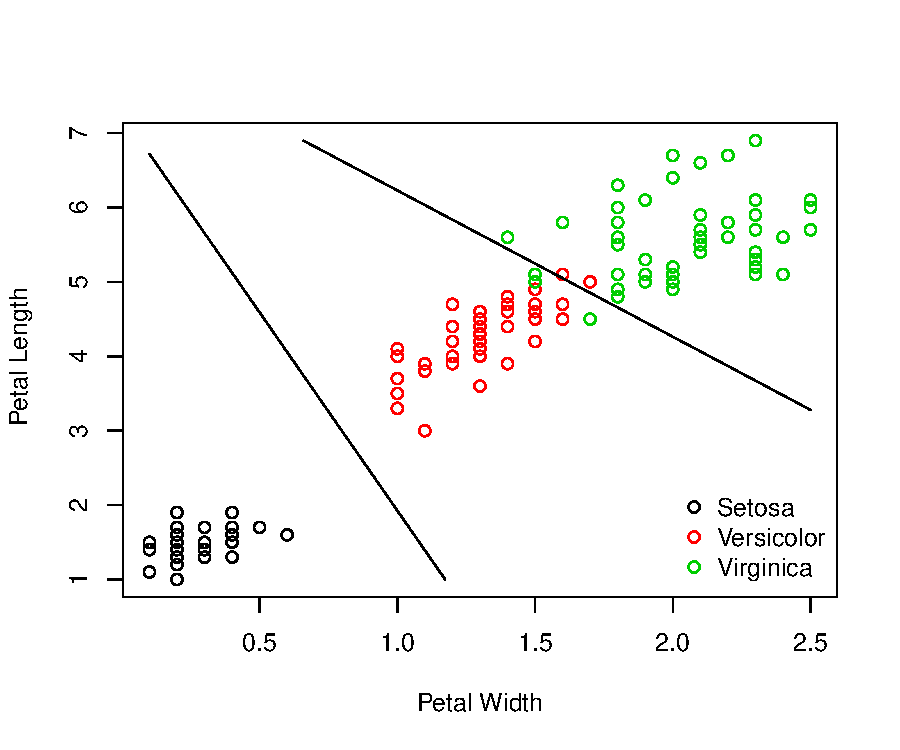
\includegraphics[width=1.6in]{lda.pdf}
\end{center}
\vspace{-8pt}
This looks nice (seems that the observations are separated into
classes), but what exactly is being shown? More next time...
\end{frame}

\begin{frame}
\frametitle{Recap: linear regression of indicators, linear
discriminant analysis}
\smallskip
In this lecture, we introduced the task of {\red classification},
a prediction problem in which the outcome is categorical

\bigskip
We can perform classification for any total number of classes $K$ by simply 
performing $K$ separate {\red linear regressions} on the appropriate 
{\red indicator vectors} of class membership.
However, there can be problems with this---when $K>2$,
a common problem is masking, in which one class is never
predicted at all

\bigskip
{\red Linear discriminant analysis} also draws linear decision 
boundaries but in a smarter way. Statistical decision theory tells
us that we really only need to know the class conditional densities
and the prior class probabilities in order to perform classification.
Linear discriminant analysis assumes normality of the data within
each class, and assumes a common covariance matrix; it then replaces
all unknown quantities by their sample estimates

\smallskip
\end{frame}

\begin{frame}
\frametitle{Next time: more linear discriminant analysis; logistic 
regression}
\smallskip
\smallskip
Logistic regression is a natural extension of the ideas behind linear
regression and linear discriminant analysis.
\smallskip
\begin{center}
\includegraphics[width=2.5in]{logr.pdf}
\end{center}
\end{frame}


\end{document}


